\documentclass{article}
\usepackage[paper=letterpaper,total={7.0in,9.4in}, top=0.7in, left=.1in]{geometry}

\usepackage{tikz}
\usepackage{verbatim}
\usepackage{listings}
\usepackage{tkz-graph}
\usetikzlibrary{calc}
%colors
\definecolor{lt-blue}{RGB}{100,100,255}
\definecolor{lt-green}{RGB}{100,255,100}

%Objects
%PERSON
\newcommand{\Person}[4]{
	\begin{scope}[xshift=#1 cm,yshift=#2 cm,xscale=#3,scale=#4]
		%head
		\draw[very thick,fill=white](2,2) circle(1);
		%eye
		\draw[very thick](2.5,2.2) circle(.1);
		%mouth
		\draw[very thick](2,1.5)--(2.83,1.5);
		%chest
		\draw [very thick](2,1)--(2,-1.5);
		\draw [very thick](2,-1.5)--(2,-4);
		%arms
		\draw [very thick,line width=2 pt,blue](2,0)--(3.2,-1.4);
		\draw [very thick,line width=2 pt,blue](2,0)--(0.8,-1.4);
		%legs
		\draw [very thick,red](2,-4)--(3.2,-5.4);
		\draw [very thick,red](2,-4)--(.8,-5.4);
		%dust
		\draw [gray](.7,-5.4)--(.3,-5.2);
		\draw [gray](.7,-5.3)--(.3,-5.0);
		\draw [gray](.7,-5.5)--(.3,-5.4);	
\end{scope}	
}
%CAR
\newcommand{\Car}[5]{

	\begin{scope}[xshift=#1 cm,yshift=#2 cm,xscale=#3,scale=#4]
		%grid to draw car on
		%\draw (-5 ,-5) grid(10 ,5);
		%\node at (0,0) {0,0};
		%body
		\draw[line width = 2pt](0,-4)--(4,-4);
		\draw[line width=2pt] (0 ,-4) arc (0:180:1); 
		\draw[line width=2pt] (6 ,-4) arc (0:180:1);
		%color empty space
		\draw [#5,ultra thin,fill = #5] (-2 ,-3.96) rectangle (6 ,-2.17); 
		\draw[#5,ultra thin,fill=#5] (-1.7,-2.2).. controls (5.5,-1.8) and (7,-2) ..(5.5,-2.2);
		
		%wheels
		\foreach \i in {-1,5}{
			\draw[fill=black](\i,-4) circle(.9);
			\draw[fill=white](\i,-4) circle(.5);
			\draw[fill=black](\i,-4) circle(.25);
		}
		
		%rims	%thanks to Dr.Williams for this idea
		\foreach \i in {-1,5}{
			\begin{scope}[xshift= \i cm, yshift=-4cm]
				\foreach \r in {40,80,120,...,360} { 
					\draw[rotate=\r, scale= .25, thick] (0.5,3)--(0.5,-3);
				}
			\end{scope}
		}
		
		%front bumper
		\draw [thick, fill = #5, line width=2pt](-2 ,-4)..controls(-4.7 ,-4) and (-3 ,-2)..(-1.7 ,-2.2);
		\draw [thick, fill = #5, line width=2pt](-1.7 ,-2.2)..controls(-1.3 ,-2.5)..(-1.2 ,-3);
		
		%screen and roof
		%\draw [thick, red, line width=2pt](-1.7 ,-2.2)..controls(-1 ,-2.1) and (0.5 ,-.5)..(.8 ,-.5);
		\draw [thick, fill = #5, line width=2pt](-1.7 ,-2.2)..controls(1 ,1) and (5.5 ,1)..(5.5 ,-2);
		
		%back bumper
		\draw [thick, fill = #5, line width=2pt](6 ,-4)..controls( 7.3,-4.3) and (7 ,-1)..(5.5 ,-2);
		\draw [thick,fill = #5, line width=2pt](5.5 ,-2)..controls(5.1 ,-2.3)..(5 ,-3);
		
		%windows
		\draw [thick, line width=2pt](-.5,-2.1)..controls(1 ,-1.9) and (3.8,-1.9)..(4.5 ,-2);
		\draw [thick, line width=2pt,fill = cyan, nearly opaque](-.5,-2)..controls(.5 ,-.8) and (4.4,1)..(4.5 ,-1.9);
		\draw [thick, line width=2pt](-.5,-2.1)..controls(.5 ,-.8) and (4.4,1)..(4.5 ,-2);
		
		%door
		\draw [thick,line width=2pt](2.2,.2)..controls(2,-2.5)..(2 ,-4);
		
		%lights
		%front
		\draw [thick,line width=2pt,fill=yellow](-3,-2.56)..controls(-2.5,-3) and(-2.5,-3.5)..(-3.45 ,-3.3);
		%back
		\draw [thick,line width=2pt,fill=yellow](6.6,-2.2)..controls(6.1,-2.5) and(6.1,-2.7)..(6.8 ,-2.8);
		
		%door knobs
		%front
		\draw[thick,fill = #5,line width=2pt](1.6,-2.2)--(1.6 ,-2.5);
		\draw[thick,fill = #5,line width=2pt](1.6,-2.2)..controls(1.2,-2.2) and (1.1,-2.5)..(1.6 ,-2.5);
		%back
		\draw[thick,fill = #5,line width=2pt](3.4,-2.2)..controls(3.7,-2.2) and (3.7,-2.5)..(3.4 ,-2.5);
		\draw[thick,fill = #5,line width=2pt](3.4,-2.2)..controls(3.1,-2.2) and(3.1,-2.5)..(3.4 ,-2.5);
		
		%rearview mirror
		%base
		\draw[thick,fill = #5,line width=2pt] (-.3,-2) circle(.13);
		\draw[thick,fill = #5,line width=2pt](-.3,-2).. controls (.9,-1.1) and (.4,-2.5) ..(-.3 ,-2);
	\end{scope}
}
%STREET
\newcommand{\Street}[3]{
	\begin{scope}[xshift=#1 cm,yshift=#2 cm,scale=#3]
	%SideWalk
	\foreach \x in {-5,-2.75,...,6.25}{
		\foreach \y in {3.8,-8}{
			\begin{scope}[xshift=\x cm,yshift=\y cm,scale=.5]
				\draw[ gray ,fill = gray!10 ] (-.5,-7) rectangle (5 ,-2);
				\draw[ gray ,fill = gray!10 ] (-.5,-7.6) rectangle (5 ,-7);
			\end{scope}
		}		
	}
	%Road
	\begin{scope}
		\draw[ gray ,fill = gray ] (-5.27,-9) rectangle (8.8 ,0);
		%white lines
		\foreach \x in{-4,0,4}{
			\draw[ black ,fill = white!90!black ] (\x,-4.5) rectangle (\x+3 ,-3.9);
		}
		
	\end{scope}
	\end{scope}
}
%Road
\newcommand{\road}[3]{	
	\begin{scope}[xshift=#1 cm, yshift=#2 cm, scale=#3]
		\draw[ gray ,fill = gray ] (-5.27,-9) rectangle (8.8 ,0);
		%white lines
		\foreach \x in{-4,0,4}{
			\draw[ black ,fill = white!90!black ] (\x,-4.5) rectangle (\x+3 ,-3.9);
		}
		
\end{scope}}

%#########################################################################
%#########################################################################
\title{Tikz Examples}
\author{Daniel Alvarez}
\begin{document}
\maketitle

\section{Cartoon art in Tikz}
\subsection{Stick Figures}
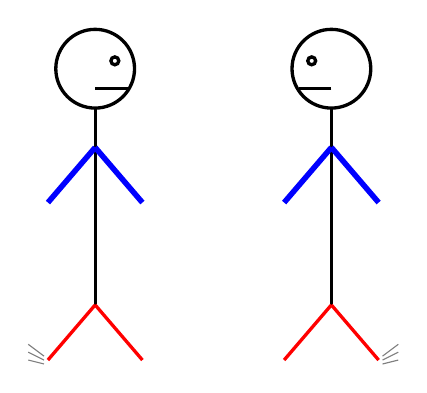
\begin{tikzpicture}
%one person
\Person{5}{0}{1}{.5}
\Person{10}{0}{-1}{.5}

\end{tikzpicture}
\vspace{.3in}
% % % % % % % % % % % % % % % % % % % % % % % % % % % % % % % % % % % % % % % % % % % % % % % % % 
\subsection{Cars}
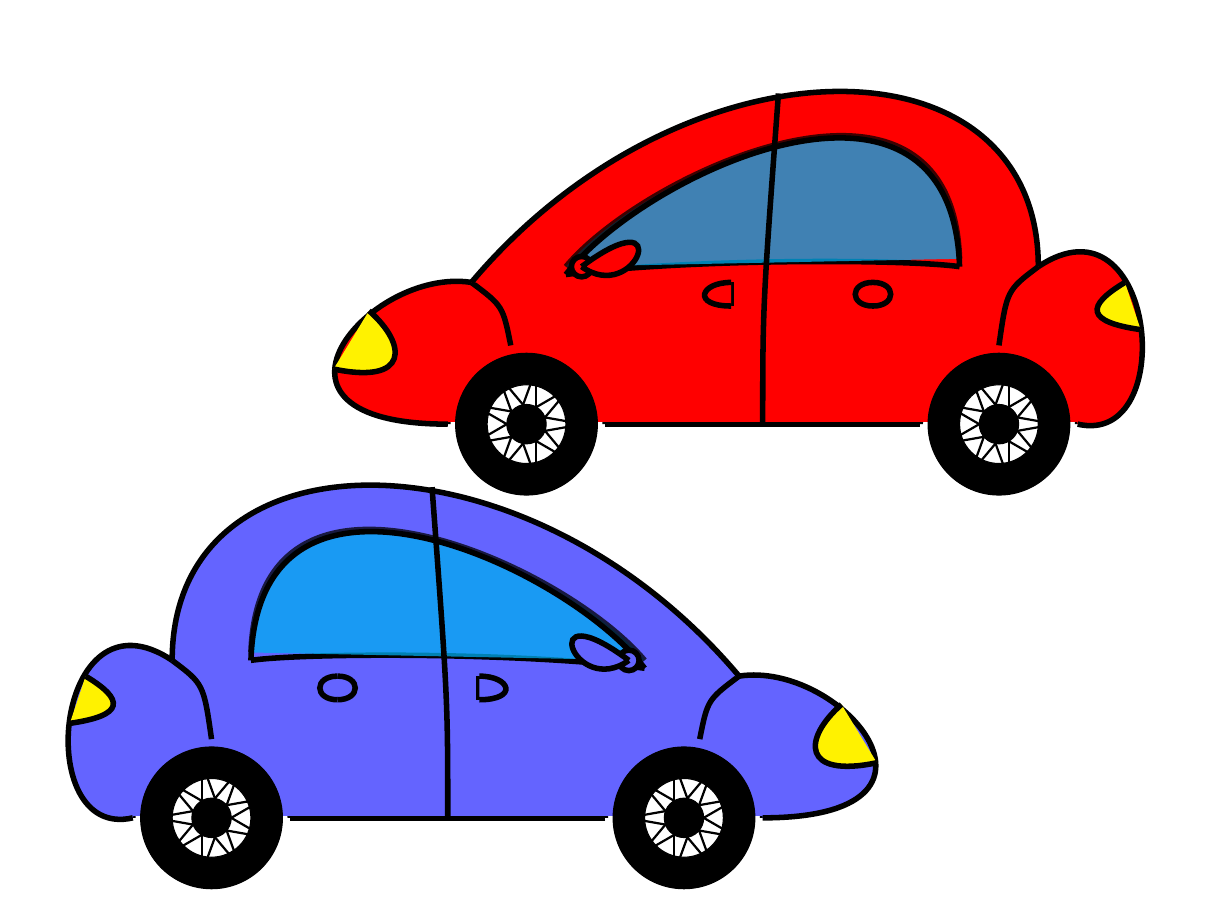
\begin{tikzpicture}

\Car{0}{0}{1}{1}{red}
\Car{0}{-5}{-1}{1}{lt-blue}
\end{tikzpicture}
% % % % % % % % % % % % % % % % % % % % % % % % % % % % % % % % % % % % % % % % % % % % % % % % % 
\section{Multiple cars}
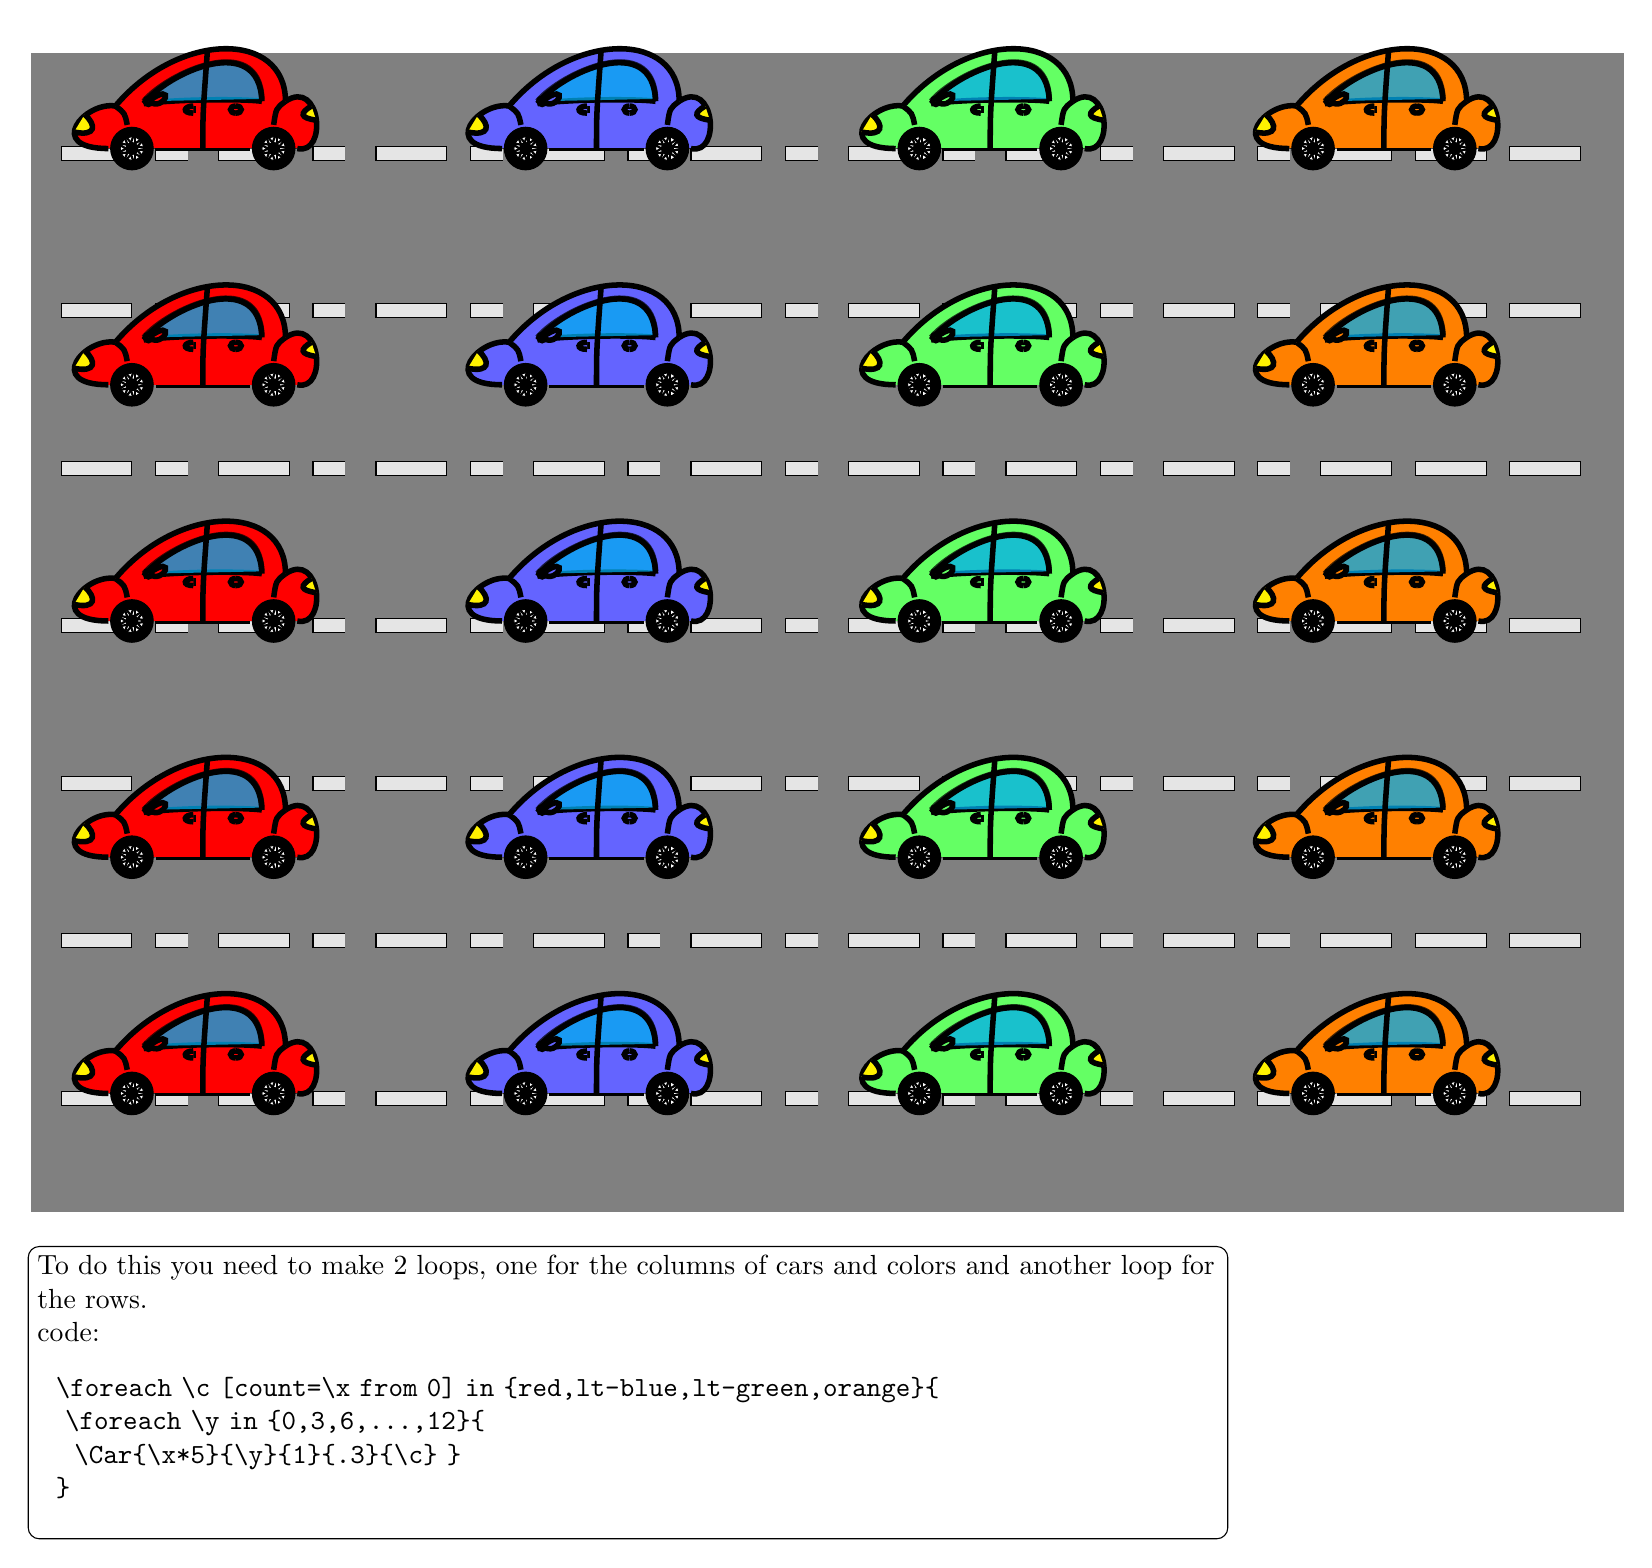
\begin{tikzpicture}

	\foreach \x in{0,2,...,16}{
		\foreach \y in{0,2,4,...,12}	{
			\road{\x}{\y}{.3}
	}
}
	\foreach \c [count=\x from 0] in {red,lt-blue,lt-green,orange}{
		\foreach \y in {0,3,6,...,12}{
			\Car{\x*5}{\y}{1}{.3}{\c}
		 }
		}
	
\node [draw , rectangle, rounded corners,text width=15 cm] at (6 ,-5) { 
	To do this you need to make 2 loops, one for the columns of cars
	and colors and another loop for the rows.\\
	code:
	\begin{verbatim}
		\foreach \c [count=\x from 0] in {red,lt-blue,lt-green,orange}{
			\foreach \y in {0,3,6,...,12}{
				\Car{\x*5}{\y}{1}{.3}{\c} } 
		}
	\end{verbatim}
	 };

\end{tikzpicture}

\subsection{Street Scene}
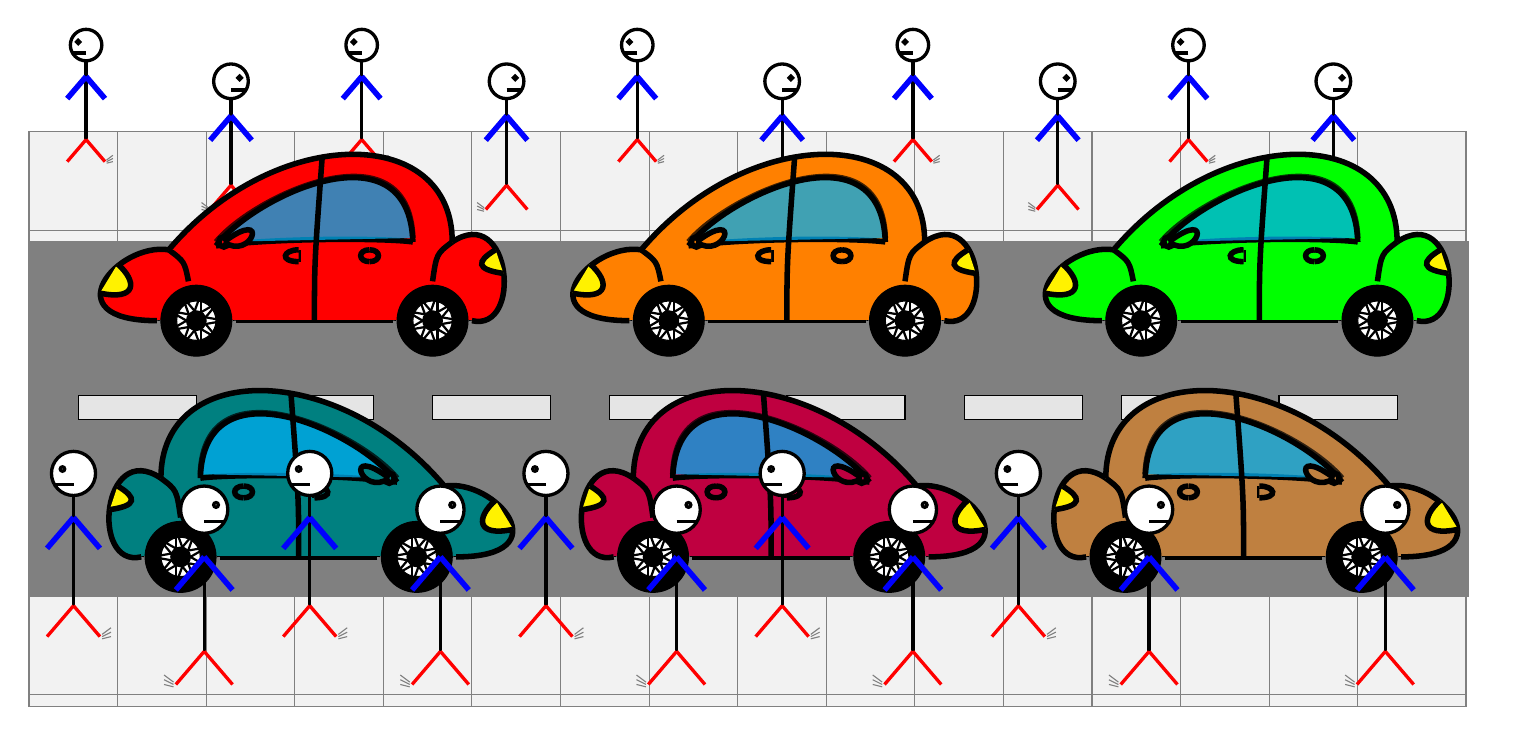
\begin{tikzpicture}
%Street
\foreach \i in {0,2.25,4.5,...,11.5}{
	\Street{\i}{0}{.5}
}
%Top People
%pedestrians walking left
\foreach \x in {-1.5,2,...,14}{
	\Person{\x}{2.1}{-1}{.2}	
}

%pedestrians walking right
\foreach \x in {-.5,3,...,15}{
	\Person{\x}{1.6}{1}{.22}	
}

%top lane
\foreach \c [count=\x from 0] in {red,orange,green}{
		
		\Car{\x*6}{1}{1}{.5}{\c}
	}
%bottom lane
\foreach \c [count=\x from 0] in {teal,purple,brown}{
	
	\Car{(\x+.3)*6}{-2}{-1}{.5}{\c}
}


%Bottom People
%pedestrians walking right
\foreach \x in {-1,2,...,14}{
	\Person{\x}{-4}{1}{.3}	
}
%pedestrians walking left
\foreach \x in {-1.5,1.5,...,12}{
	\Person{\x}{-3.5}{-1}{.28}	
}	


\end{tikzpicture}
\vspace{1 in}

\section{Playing with rotations}

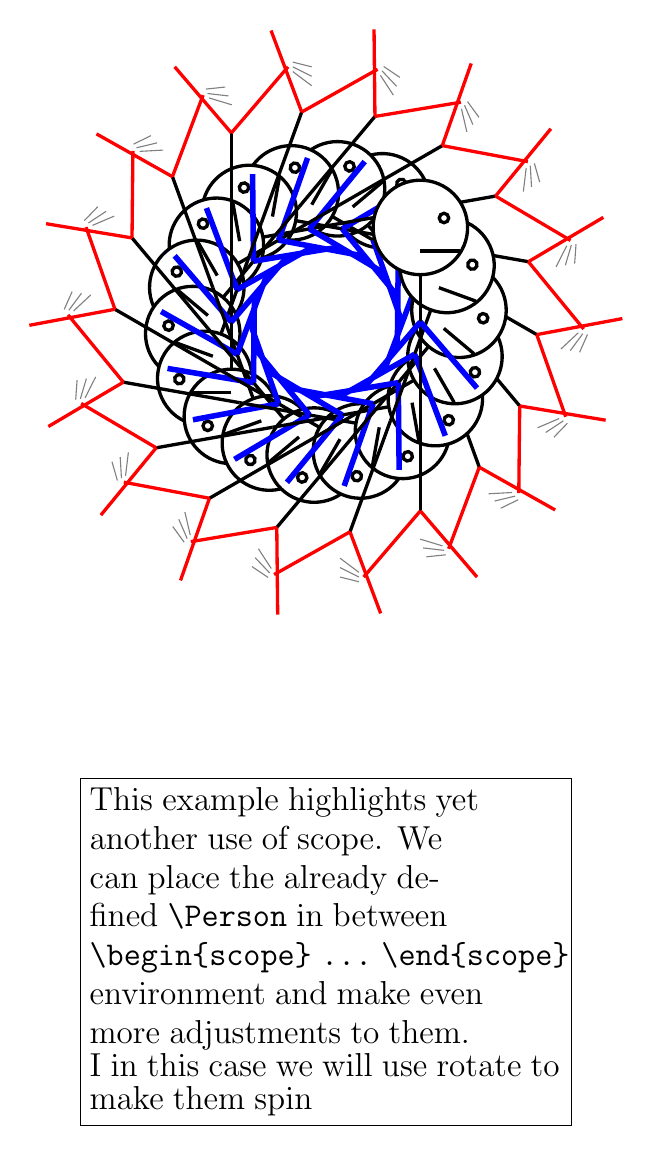
\begin{tikzpicture}
\node[,draw,text width= 6cm,scale=1] at (0,-8){
	\large{This example highlights yet another use of scope. 
	We can place the already defined 
	\verb|\Person| in between \verb|\begin{scope} ... \end{scope}|
    environment and make even more adjustments to them.\\
I   in this case we will use rotate to make them spin}};

\foreach \r in {20,40,...,360}{

\begin{scope}[rotate = \r]

\Person{0}{0}{1}{.6}
\end{scope}
}
\end{tikzpicture}
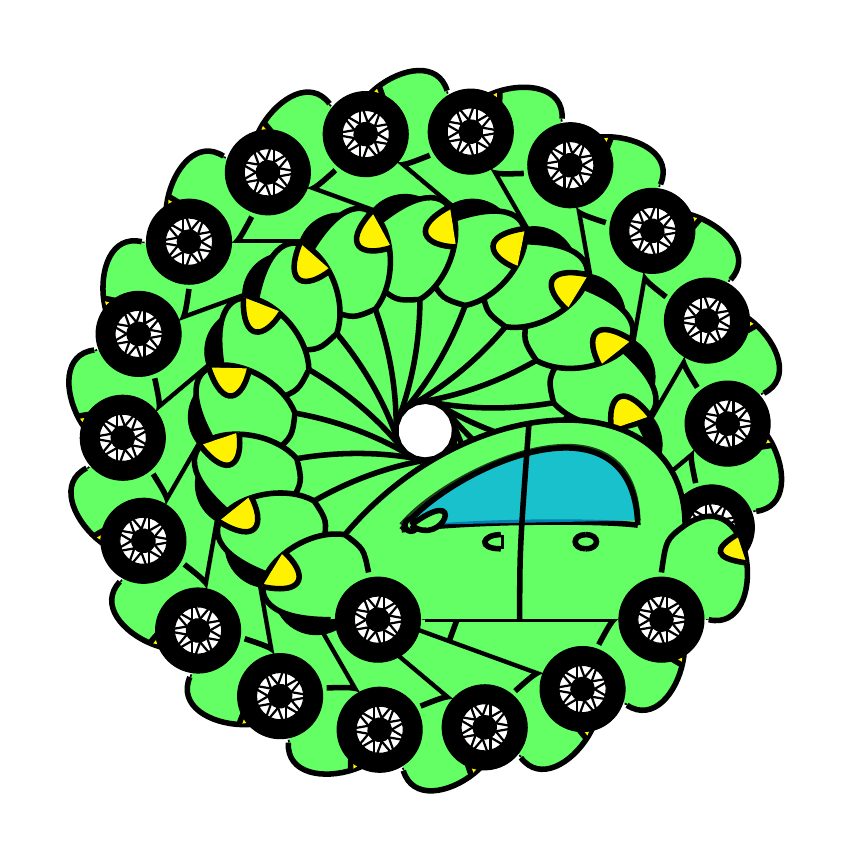
\begin{tikzpicture}
	
		\foreach \r in {20,40,...,360}{
			\begin{scope}[rotate = \r]
				\Car{0}{0}{1}{.6}{lt-green}
			\end{scope}
		}	
	
\end{tikzpicture}
\vspace{1 in}
\section{spinning}
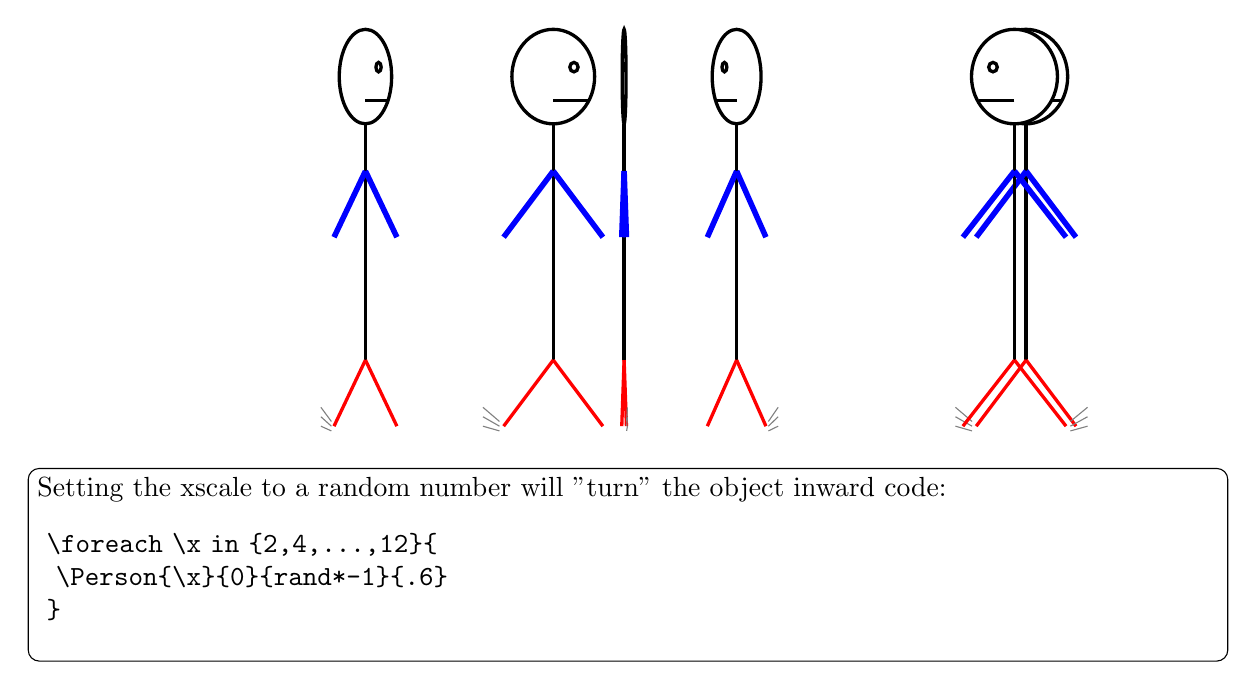
\begin{tikzpicture}
	\foreach \x in {2,4,...,12}{
		
		\Person{\x}{0}{rand*-1}{.6}
	}	
\node [draw , rectangle, rounded corners,text width=15 cm] at (6 ,-5) { 
	Setting the xscale to a random number will "turn" the object
	inward
	code:
	\begin{verbatim}
	\foreach \x in {2,4,...,12}{
		\Person{\x}{0}{rand*-1}{.6}
	}	
	\end{verbatim}
};
\end{tikzpicture}
\section{Varying scale}
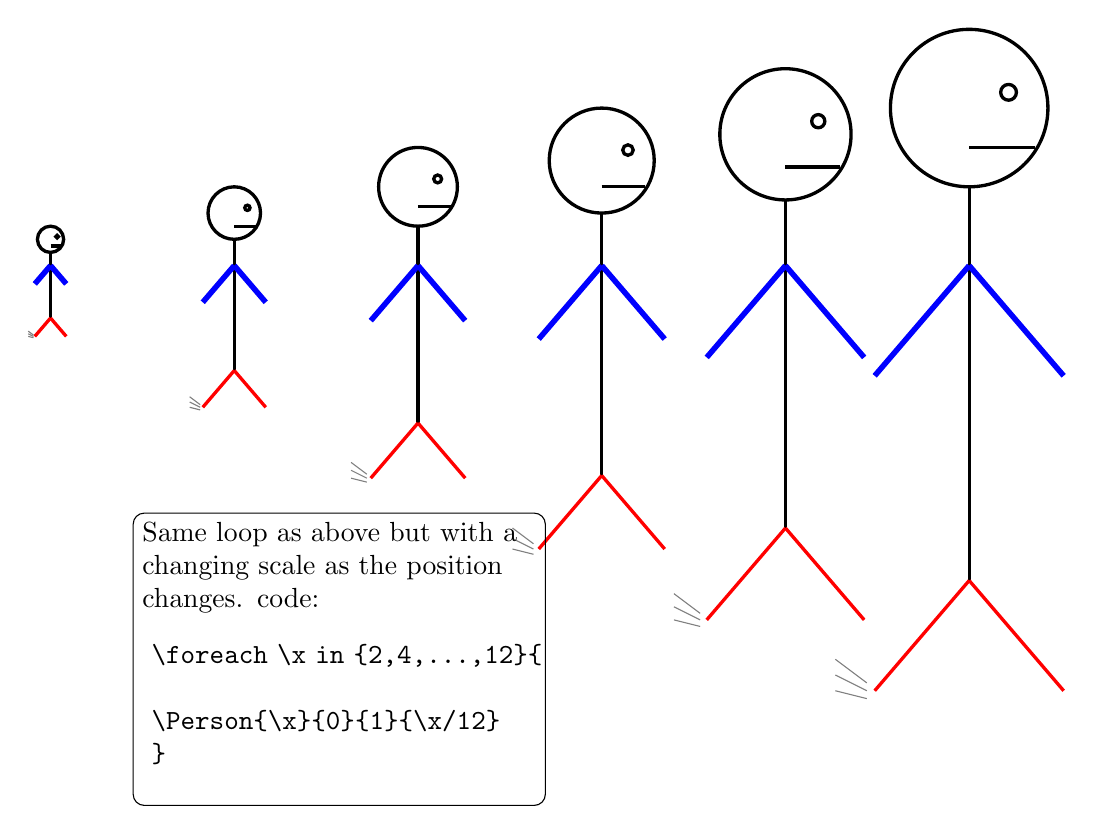
\begin{tikzpicture}
\foreach \x in {2,4,...,12}{
	
	\Person{\x}{0}{1}{\x/12}
}	
\node [draw , rectangle, rounded corners,text width=5 cm] at (6 ,-5) { 
	Same loop as above
	but with a changing scale as
	the position changes.
	code:
	\begin{verbatim}
	\foreach \x in {2,4,...,12}{
	
	\Person{\x}{0}{1}{\x/12}
	}	
	\end{verbatim}
};
\end{tikzpicture}

\section{Varying shades}
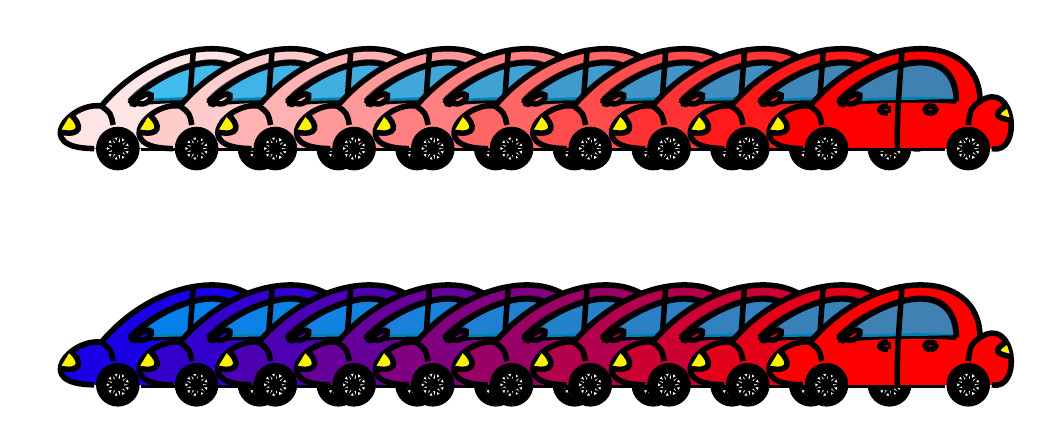
\begin{tikzpicture}
\foreach \c [count=\x from 0] in {10,20,...,100}{
		\Car{\x}{0}{1}{.3}{red!\c!white}
}
\foreach \c [count=\x from 0] in {10,20,...,100}{
	\Car{\x}{-3}{1}{.3}{red!\c!blue}
}

\end{tikzpicture}
\section{Combining Things}
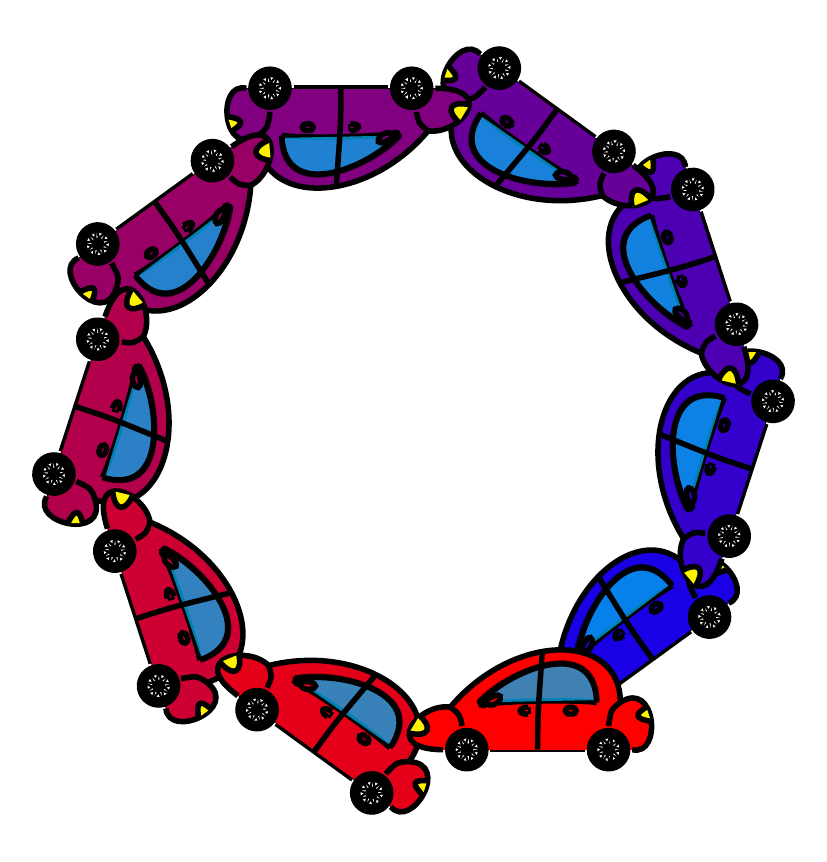
\begin{tikzpicture}
	\foreach \c [count=\x from 0] in {10,20,...,100}{
		\begin{scope}[rotate = \c*3.6]
		\Car{\x*.1}{-3}{1}{.3}{red!\c!blue}
		\end{scope}
	}

\end{tikzpicture}

\end{document}